\documentclass{article}

\usepackage[french]{babel}
\usepackage[utf8]{inputenc}
\usepackage[]{amsmath}
\usepackage{graphicx}
\usepackage{subcaption}
\usepackage{hyperref}

%%%%%%%%%%%%%%%% Lengths %%%%%%%%%%%%%%%%
\setlength{\textwidth}{15.5cm}
\setlength{\evensidemargin}{0.5cm}
\setlength{\oddsidemargin}{0.5cm}

%%%%%%%%%%%%%%%% Variables %%%%%%%%%%%%%%%%
\def\projet{4}
\def\titre{Systèmes d'équations non-linéaires / Méthode de Newton-Raphson}
\def\groupe{4}
\def\equipe{3}
\def\responsible{mrekik018}
\def\secretary{jeamartinez}
\def\others{scomiti, aguerouani, acattarin}

\begin{document}

%%%%%%%%%%%%%%%% Header %%%%%%%%%%%%%%%%
\noindent\begin{minipage}{0.98\textwidth}
  \vskip 0mm
  \noindent
  { \begin{tabular}{p{7.5cm}}
      {\bfseries \sffamily
        Projet \projet} \\ 
      {\itshape \titre}
    \end{tabular}}
  \hfill 
  \fbox{\begin{tabular}{l}
      {~\hfill \bfseries \sffamily Groupe \groupe\ - Equipe \equipe
        \hfill~} \\[2mm] 
      Responsable : \responsible \\
      Secrétaire : \secretary \\
      Codeurs : \others
    \end{tabular}}
  \vskip 4mm ~

  ~~~\parbox{0.95\textwidth}{\small \textit{Le but de ce projet est d'implémenter des algorithmes de recherche de racine de systèmes d'équatiosn non linéaire. Ensuite, nous appliquerons ces algorithmes à des problèmes concrets, choisit parmis la liste de sujets proposés.} \sffamily }
  \vskip 1mm ~
\end{minipage}

%%%%%%%%%%%%%%%% Main part %%%%%%%%%%%%%%%%
\section{Newton-Raphson solver}
\subsection {Question 1} 
Puisque $f(U+V)=0$ et étant donné l'approximation,on a
\newline
 $f(U)+H(U)*V=0$

\subsection{Question 3}

Une manière simple de tester la fonction dans le cas où $f$ est une fonction de $R$ dans $R$ est de prendre $f(x)=x^2-4$ et $x_0=1.1$. On choisit également le nombre d'itération N et le seuil de convergence epsilon. On obtient alors le résultat suivant:
\newline
$x_sol=2.0$

\section{Applications}
\subsection{Computation of the Lagrangian points}
Dans cette partie, nous nous plaçons dans une situation où deux forces gravitationnelles de coefficients 1 (resp. 0.01) centrées en $[0, 0]$ (resp. $[1, 0]$)

Une troisième force, centrifuge, de coefficient 1 et centrée sur le barycentre des deux précédentes. Ce point $(x, y)$ peut être trouvé en résolvant le système suivant :

$$
\begin{cases}
  a(A_x - x) + b(B_x - x) = 0 \\
  a(A_y - y) + b(B_y - y) = 0
\end{cases}
$$

avec $a$ et $(A_x, A_y)$ (resp. $b$ et $(B_x, B_y)$) respectivement le coefficient et le point d'application de la première (resp. deuxième) force gravitationnelle décrite précédemment.

Après résolution, on obtient $x = \frac{0,01}{1,01}$ et $y = 0$ comme coordonnées du point d'application de la force centrifuge.

\bigskip

Afin de calculer les points d'équilibre de ce système, nous allons utiliser plusieurs fois l'algorithme implémenté dans la partie \ref{sec:newton}. Après plusieurs itérations de l'algorithme en utilisant des points initiaux différents, on obtient cinq points d'équilibres : \emph{P1} = [0,5  0,870], \emph{P2} = [0,5  -0,870], \emph{P3} = [-0,998  0], \emph{P4} = [0,859  0], \emph{P5} = [1,158  0].

Ces points sont représentés sur la figure \ref{fig:equi_pts} :

\begin{figure}[ht]
  \centering
  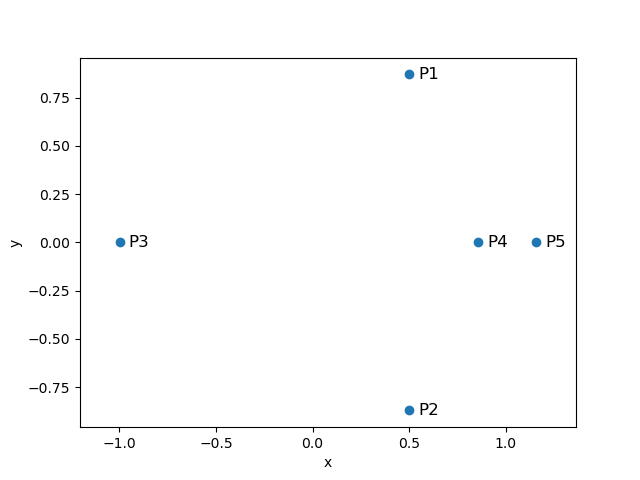
\includegraphics[width=0.5\textwidth]{img/equilibrium_points.png}
  \caption{Les différents points d'équilibre dans la plan de la situation décrite dans la partie \ref{ssec:lagrange}}
  \label{fig:equi_pts}
\end{figure}

\bigskip

Cette situation est celle d'une planète étant en orbite autour d'une étoile. Ici, la masse en position $[0, 0]$ est l'étoile, et celle en position $[1, 0]$ est la planète. Les points de Lagrange sont les points d'équilibre pour un objet de petite masse (par exemple un satellite) qui serait sous l'influence, dans notre cas, d'une étoile et d'une planète gravitant autour d'elle. Les points d'équilibre que nous avons calculer précédemment sont donc les points de Lagrange de ce cas-ci.

En modifiant les valeurs des coefficients et des points d'applications des forces, on obtient d'autres points d'équilibre : les points de Lagrange. Il est important de rappeler que leurs coordonnées ne sont pas les coordonnées exactes. Elles sont obtenues avec une précision de 0.01 dans notre cas.

\bigskip

Nous pouvons vérifier nos résultats en les comparant avec les points de Lagrange dans la situation où la Terre orbite autour du Soleil. Ces points sont donnés dans la figure \ref{fig:lagr_pts}. Ces points sont en concordance avec nos résultats présents en figure \ref{fig:equi_pts}.

\begin{figure}[ht]
  \centering
  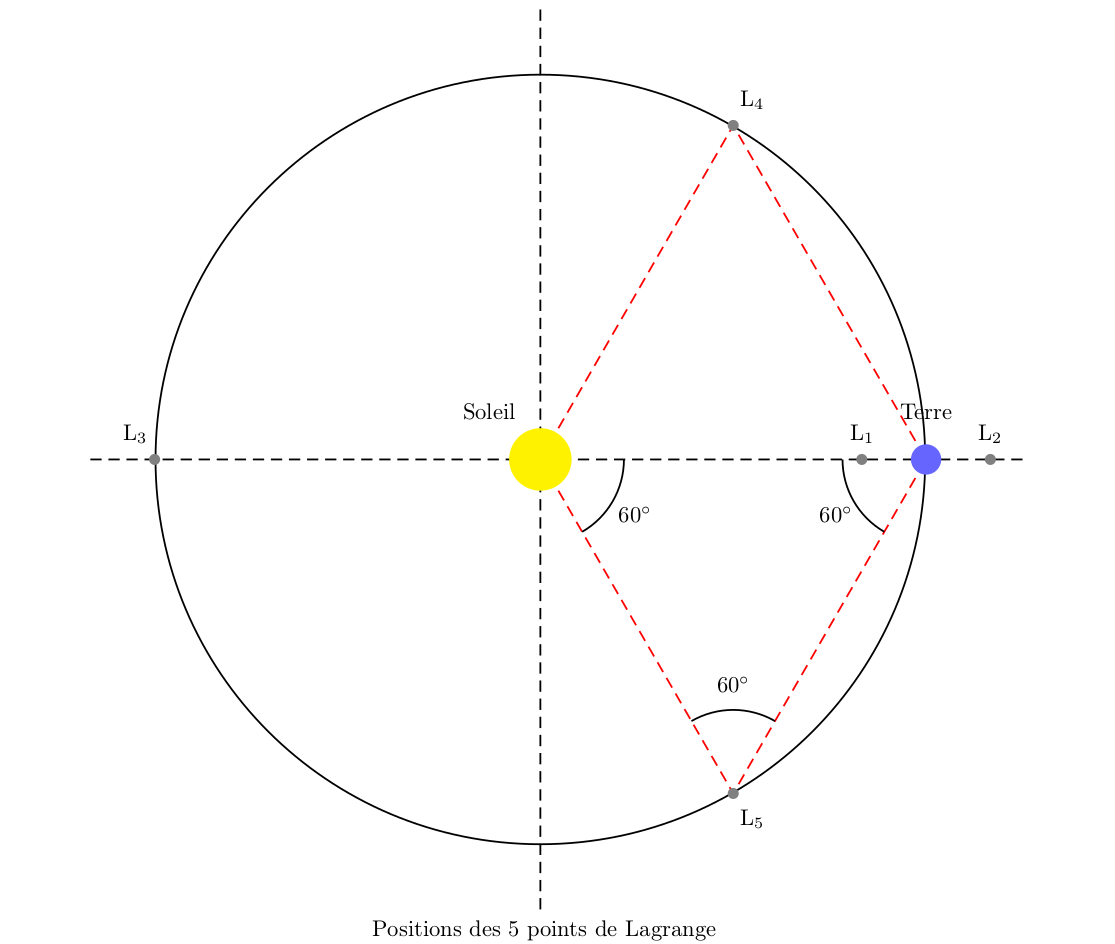
\includegraphics[width=0.5\textwidth]{img/lagrangian_points.png}
  \caption{Les points de Lagrange (L1...L5) dans le cas où la Terre orbite autour du Soleil}
  \label{fig:lagr_pts}
\end{figure}

\subsection{Electrostatic equilibrium}
Dans cette partie nous allons apliquer la méthode de résolution de Newton-Raphson afin de trouver l'équilibre électrostatique d'un système constitué de $N$ charges libres se situant aux positions $x_{1},x_{2},...,x_{N}$ dans l'intervale $[-1,1]$. Notre objectif est donc de déterminer un extremum de la fonction de l'énergie totale du système $E$ qui s'exprime par:
\begin{equation}
  E(x_{1},x_{2},...,x{N}) =  \summation{N}{i=1}(log|x_{i}+1| + log|x_{i} -1 + \frac{1}{2}\summation{N}{j=1,j \neq i} log|x_{i} - x{j}| 
\end{equation}
Cela ce traduit par la résolution de l'équation non-linéaire :
\begin{equation}
  \label{eq:eq1}
  \begin{split}
  \nabla E(x_{1},x_{2},...,x_{N}) = 0
  \end{split}
\end{equation}

\subsection{Calcul de la matrice Jacobienne de $\nabla E$}
Après simplification de l'expression du gradient de la fonction d'énergie totale on obtient : 
\begin{equation}
  \label{eq:gradient}
  \begin{split}
    \nabla E(x_{1},x_{2},...,x_{N})  & = \left( \frac{\partial E }{\partial x_{i}}\right)_{1 \leq i \leq N} \\
    & = \left(\frac{1}{x_{i}+1} + \frac{1}{x_{i} -1} + \frac{1}{2} \summation{N}{j=1,j\neq i}\frac{1}{x_{i}-x{j}}\right)_{1 \leq i \leq N }
  \end{split}
\end{equation}
On note $J$ la matrice Jacobienne de $\nabla E$
on a d'après \ref{eq:gradient} :
\begin{equation}
  \label{eq:jacobian}
  \begin{split}
    J & = \left(\frac{\partial \nabla E }{\partial x_{i} \partial x_{j}}\right)_{1 \leq i \leq N , 1 \leq j \leq N} \\
    & = \left\{
    \begin{array}{ll}
      -\frac{1}{(x_{i}+1)^{2}} - \frac{1}{(x_{i} -1)^{2}} - \frac{1}{2} \summation{N}{j=1,j\neq i}\frac{1}{(x_{i}-x{j})^{2}}& \mbox{si i = j} \\
      -\frac{1}{2(x_{i} - x{j})^{2}} & \mbox{sinon} 
    \end{array}
    \right.
  \end{split}  
\end{equation}

En Python, les deux fonctions sont mises en œuvre et l'algorithme de Newton-Raphson est appliqué en utilisant la fonction $\nabla E(x_1, x_2, \cdots , x_N)$ et la fonction qui calcule sa Jacobienne définie par l'équation \eqref{eq:jacobian}. Le résultat est un vecteur dont les coordonnées sont les solutions de l'équation \eqref{eq:eq1}. La figure \ref{fig:legendre} illustre ces solutions placées sur l'axe des réels, avec en surimpression les dérivées des polynômes de Legendre d'ordre 1 à 6. On peut constater que les racines des dérivées correspondent approximativement aux coordonnées du vecteur solution.

\begin{figure}[H]
  \centering
  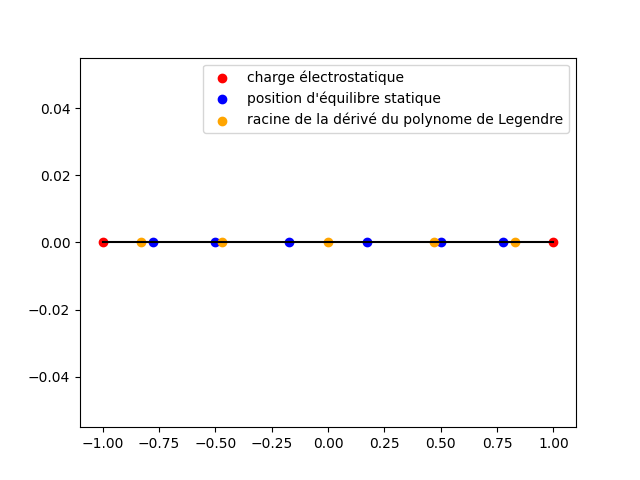
\includegraphics[width=0.5\textwidth]{img/legendre.png}
  \caption{Vecteur solution positionné sur l'axe des réels, superposé avec les racines de la dérivées des polynomes de Legendre d'ordre 1 à 6}
  \label{fig:legendre}
\end{figure}

Pour évaluer si la solution correspond à un maximum ou à un minimum, on s'est appuyé sur les valeurs propres de la matrice jacobienne $J_{\nabla E}$, calculée pour le vecteur contenant les positions d'équilibre. Étant donné que toutes les valeurs propres sont négatives, on peut conclure que la solution correspond à un maximum.





\end{document}
